\section{Decision Theory - Optimal Strategies}
Suppose we have estimates of predictive probabilities for the outcomes of all possible matchups in the NCAA tournament. Decision theory gives us a framework to choose the optimal submission for almost any bracket competition. 

ESPN's yearly tournament challenge draws millions of March Madness fans into bracket competitions, or pools, with their friends. In some cases, these pools wager a certain amount of money, and the highest-scoring bracket wins the jackpot. Additionally, ESPN offers some prizes for the best brackets over all submissions. Most players are therefore keen on entering such competitions with a bracket that is likely to win. 

The ESPN Tournament Challenge awards points for each matchup according to the formula $10\times2^{r-1}$ where $r$ is the round in which the matchup occurs. So a correct pick for the third round will give $40$ points. Scoring is clearly done in this way so that each round has the potential of awarding a player the same number of points: 320. 

Recently in the headlines, Warren Buffet announced a prize of $\$1$ billion for the first perfectly-predicted March Madness bracket. Predicting a perfect bracket is similar to the ESPN tournament challenge in that the optimal choice requires an understanding of the underlying probabilities governing matchups between two teams. Ultimately the competitor will need to search through a discrete space to find an optimal submission. Niemi et al. (2005) also suggest using a contrarian approach to bracket selection for the ESPN challenge in order to set a submitted bracket apart from other similar brackets within the same pool. 

In general, even given the true probabilities of all possible matchups among the 64 teams in the tournament, selecting an optimal submission is not a simple problem. Suppose that in a strange year, only four teams qualify for the NCAA tournament -- teams A, B, C, and D. Further, suppose that teams A and C are number 1 seeds, so that they will respectively play against teams B and D in the first round. Table \ref{tab:hypothetical} shows possible probabilities for the outcomes of all six possible matchups. Notice that picking the highest probablity outcome at each round will give a bracket with likelihood $0.6\times0.8\times0.1=0.048$. However, picking the underdog between teams A and B will give a bracket with likelihood $0.4\times0.8\times1=0.32$. 

Clearly, the latter bracket is the highest-likelihood bracket, which illustrates the point that brackets ought not to filled out round-by-round. This motivates underdog picks and highlights the fact that the optimal process for bracket selection is not always obvious.

\begin{table}
	\centering
	\begin{tabular}{|cc|c|}
		\hline
		Team 1	&	Team 2	&	Probability of Team 1 beating Team 2 \\
		\hline
		A 		&	B 		&	0.6\\
		A 		&	C 		& 	0.1\\
		A 		& 	D 		& 	0.1\\
		B 		&	C 		&	1\\
		B 		& 	D 		&	1\\
		C 		& 	D 		& 	0.8\\
		\hline
	\end{tabular}
	\caption{\label{tab:hypothetical}}
\end{table}

\subsection{Kaggle Competition}

The Kaggle competition is scored based on a log-loss function. Submissions consist of a list of probabilities that determine the outcomes of all 2,278 pairwise matchups between the 68 teams admitted into the March Madness playoffs. Only the 63 matchups that occur during the tournament end up in the calculation of the loss function.

Suppose a competitor in the Kaggle competition is confident in her ability to estimate the probabilities of pairwise outcomes. Is it optimal, therefore, for her to submit these predicted probabilities? Or is there a benefit to adjusting the probabilities toward the extremes of 0 and 1 so that games that result in her favor give a larger reward in the loss function? On the other hand, perhaps sliding the probabilities toward the more conservative estimate of 0.5 helps to mitigate the risk of an upset. Below we show that submitting the estimated proabilites minimizes the expected log-loss function. 

As discussed above, the loss function is 
$$
L(\underline{p})=-\frac{1}{63}\sum_{i=1}^{63}\left[y_i\log(p_i)+(1-y_i)\log(1-p_i)\right]
$$
where $p_i$ is the probability submitted by the Kaggle competitor. The posterior expected value of the loss function is therefore 
$$
E_{y|D}[L(\underline{p})]=-\frac{1}{63}\sum_{i=1}^{63}\left[\tilde{p}_i\log(p_i)+(1-\tilde{p}_i)\log(1-p_i)\right]
$$
where $\tilde{p}_i$ is the posterior predictive probability governing the outcome of the $i$th game. The $i$th partial derivative is thus
$$
\frac{\partial}{\partial p_i} E_{y|D}[L(\underline{p})] = \frac{\tilde{p}_i}{p_i}-\frac{1-\tilde{p}_i}{1-p_i}.
$$
Setting these equal to zero to satisfy first order conditions gives
$$
p_i=\tilde{p}_i.
$$
We therefore see that the expected log-loss optimal submission is the posterior predictive probability of game outcomes.

However, as argued above, it may still behoove the Kaggle competitor to push the submitted probabilities toward the boundaries or the center of the interval $[0,1]$, should she have a different loss function. One way to do this would be to introduce a new parameter $\alpha \in [-1,1]$ that systematically shifts all submitted probabilities toward the center or endpoints. We propose the following method, then evaluate its performance relative to real Kaggle submissions. Define a transformation of a probability as a function of $\alpha$ according to

$$
p^\prime= \left\{ \begin{array}{lr} 
			(1+\alpha)p - 0.5\alpha, & \mbox{if $\alpha \le 0$} \\
			(1-\alpha)p, & \mbox{if $\alpha >0$ and $p < 0.5$} \\
			(1-\alpha)p + \alpha, & \mbox{if $\alpha >0$ and $p > 0.5$} \\
			0.5,  & \mbox{if $\alpha >0$ and $p = 0.5$} \\
		   \end{array} \right. . 
$$
This transformation shifts all probabilities toward 0.5 when $\alpha \le 0$, shifts them toward the endpoints when $\alpha>0$, and gives the original probabilities when $\alpha=0$.  
Applying this transformation to the 2014 Kaggle submissions and calibrating $\alpha$ to maximize each team's scores, we find some interesting results. Figure \ref{fig:alphas} shows which alpha maximizes the recalculated score for each team, plotted against their change in score. We find that for more than $75\%$ of the teams, a non-zero $\alpha$ would have improved their scores. However, the best performing teams had optimal $\alpha$ near zero, suggesting their success is most likely attributable to accurate probability estimates accross the board.

\begin{figure}
	\centering
	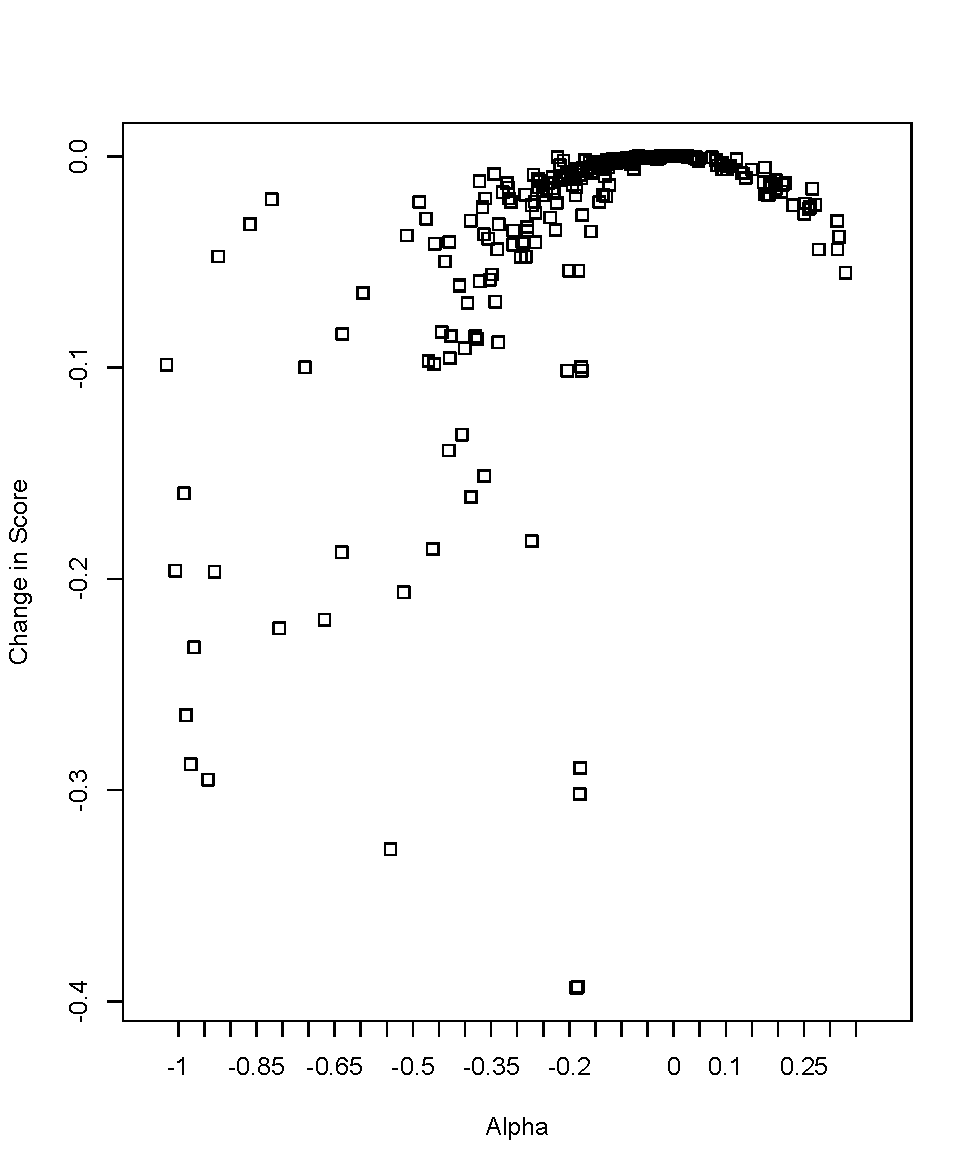
\includegraphics[width=\textwidth]{AlphaPlot.pdf}
	\caption{Kaggle team score improvements as a function of the $\alpha$ that would have maximized the scores.}
	\label{fig:alphas}
\end{figure}

The introduction of the parameter $\alpha$ to stretch or contract the estimated probabilities highlights the possibility that submitting values not equal to the actual probability estimates may be beneficial in some circumstances. To explore further, a Kaggle competitor may decide to specify a threshold, beyond which probabilities much larger (or smaller) than $0.5$ are pushed to $1$ (or $0$).
